\chapter{Cinématique en deux dimensions : Tir horizontal}
Le tir horizontal est une situation dans laquelle un objet est lancé horizontalement depuis une certaine hauteur.

\begin{figure}[h!]
    \centering
    \resizebox{\linewidth}{!}{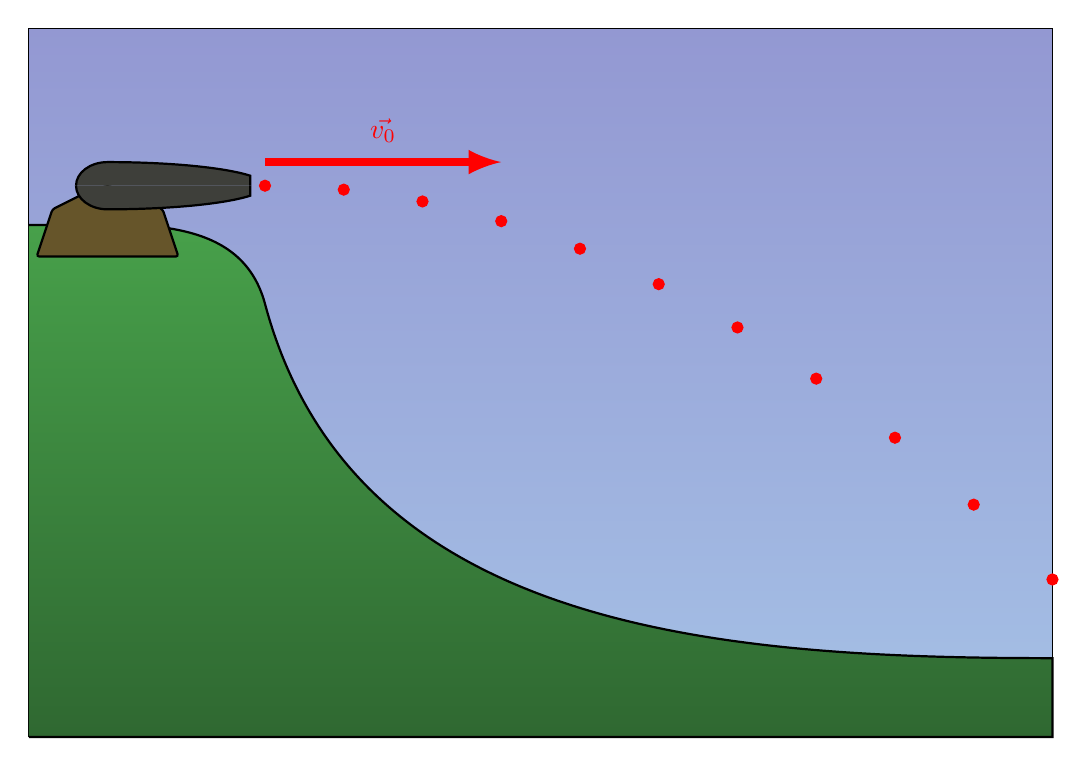
\begin{tikzpicture}
    \definecolor{sky_top}{HTML}{9398d2ff}
    \definecolor{sky_bottom}{HTML}{a5c1e6ff}
    \definecolor{support_canon}{HTML}{66552aff}
    \definecolor{canon}{HTML}{3e3f3aff}
    \definecolor{hill_top}{HTML}{48a24bff}
    \definecolor{hill_bottom}{HTML}{2f6831ff}

    \newcommand{\supportcanon}{
        \filldraw[thick,rounded corners=1pt,fill=support_canon](-9,-9) -- (-7,-3) -- (-3,-1) -- (0,0) -- (3,-1) -- (7,-3) -- (9,-9) -- cycle;
    }

    \newcommand{\canon}{
        \path (0,0) -- (12,0) node(xline){};
        \filldraw[thick,fill=canon](-4,0) arc (180:90:4cm and 3cm) arc(90:25:20cm and 3cm) coordinate(W) --(W |- xline);
        \filldraw[thick,fill=canon](-4,0) arc (180:270:4cm and 3cm) arc(270:335:20cm and 3cm) coordinate(Z) --(Z |- xline);
    }

    %dessin du ciel
    \filldraw[top color=sky_top,bottom color=sky_bottom] (-3,-7) rectangle (10,2);

    %placement de la grille
    \tkzInit[xmin=-3,xmax=10,ymin=-7,ymax=2]
    \tkzGrid

    %dessin de la colinne
    \filldraw [thick,top color=hill_top,bottom color=hill_bottom] [in=105, out=0] (-3,-0.5) to (0,-1.5) [in=180, out=-75] to  (10,-6)--(10,-7)--(-3,-7);

    %placement des axes
    \tkzDrawXY

    %placement du canon et du support
    \begin{scope}[shift={(-2,0)},scale=.1]
        \supportcanon
        \canon
    \end{scope}

    %placement des points représentant la trajectoire du boulet
    %V0=10[m/s]
    %enX : x(t)=10*t
    %enY : y(t)=-4.905*t
    \foreach \t in {0,0.1,...,1.1}
        {\pgfmathsetmacro{\x}{10*\t}
            \pgfmathsetmacro{\y}{-5*\t*\t}
            \filldraw [red] (\x,\y) circle (2pt);
        }

    %le vecteur vitesse initiale
    \draw[->,>=latex,color=red,line width=3pt](0,0.3) -- (3,0.3);
    \node at (1.5,0.7)[color=red] {\(\vec{v_0}\)};

    %les commentaires
    \tkzText[draw, color=black,fill=lightgray,text width=5cm](6,1){Le mouvement horizontal est un MRU}
    \tkzText[draw, color=black,fill=lightgray,text width=5cm](0,-6){Le mouvement vertical est un MRUA}
\end{tikzpicture}}
    \caption{Schéma d'un tir horizontal.}
    \label{Schéma d'un tir horizontal}
\end{figure}

\section{Indépendance des mouvements en deux dimensions}
La photo ci-dessous est une chronophotographie présentant deux corps laissés en chute libre au même instant. Celui de gauche possède une vitesse en X non nulle, il s'agit donc d'un tir horizontal.
\begin{figure}[h!]
    \centering
    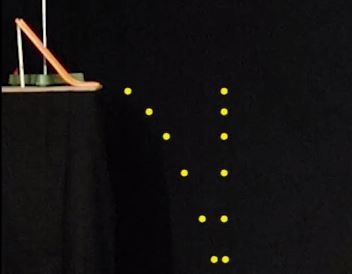
\includegraphics[width=.5 \linewidth]{chronophoto_tir_horizontal.jpg}
    \caption{Chronophotographie d'un tir horizontal comparé à une chute libre.}
    \label{chronophoto_tir_horizontal}
\end{figure}
Cette image montre que les deux corps tombent en même temps, la seule différence est que celui de gauche avance en même temps qu'il tombe.


\begin{encadre}
    Dans un mouvement à deux dimensions, le mouvement horizontal est totalement indépendant du mouvement vertical. Le mouvement vertical est celui d'une chute libre : un MRUA causé par l'accélération de la pesanteur terrestre.
    L'accélération étant uniquement dirigée vers le bas, le mouvement horizontal du corps est celui d'un MRU.
\end{encadre}

\newpage

\section{Le vecteur vitesse dans un mouvement à deux dimensions}
À un moment donné de sa trajectoire, le mobile possède à la fois une vitesse horizontale, \(\vec{v_x}\), et une vitesse verticale, \(\vec{v_y}\). La vitesse totale du mobile à un instant quelconque est donc donnée par la somme vectorielle de la vitesse horizontale et de la vitesse verticale. Cette somme se fait en utilisant le théorème de Pythagore : \(v_{tot}=\sqrt{v_x ^2 + v_y ^2}\)

\begin{tikzpicture}
    \tikzset{>=latex}
    \tkzDefPoint(0,0){o}
    \tkzDefPoint(3,0){a}
    \tkzDefPoint(0,-4){b}
    \tkzDefPoint(3,-4){c}

    \tkzMarkRightAngle[size=.3,fill=lightgray,opacity=.5](o,b,c)

    \tkzDrawSegment[->,line width=2pt,color=ForestGreen](o,a)
    \tkzLabelSegment[above,color=ForestGreen](o,a){\(\vec{v_x}\)}
    \tkzDrawSegment[line width=1pt,color=ForestGreen,opacity=0.5,style=dotted](b,c)

    \tkzDrawSegment[->,line width=2pt,color=NavyBlue](o,b)
    \tkzLabelSegment[right,color=NavyBlue](o,b){\(\vec{v_y}\)}
    \tkzDrawSegment[line width=1pt,color=NavyBlue,opacity=0.5,style=dotted](a,c)

    \tkzDrawSegment[->,line width=2pt,color=BrickRed](o,c)
    \tkzLabelSegment[right=3pt,color=BrickRed](o,c){\(\vec{v_{tot}}\)}
\end{tikzpicture}

\section{Exercices}
\begin{exercise}
    Un objet est lancé horizontalement depuis une hauteur de \(6\unit{[m]}\) et avec une vitesse de \(4\unit{[m/s]}\).
    \begin{enumerate}[label=\alph*)]
        \item Combien de temps prend-il pour atteindre le sol ?
        \item Quelle distance parcoure-t-il horizontalement avant de toucher le sol ?
        \item Quelle est sa vitesse totale à l'impact ?
    \end{enumerate}
\end{exercise}

\begin{exercise}
    Quelle doit être la vitesse initiale d'un projectile lancé horizontalement depuis une hauteur de \(25[m]\) pour qu'il atteigne le sol à une distance horizontale de \(40[m]\) par rapport à sa position de départ ?

    Quelle sera sa vitesse totale à l'impact ?
\end{exercise}
\begin{solution}
    \(t_{chute}=2,258[s]\)
    \(v_{y ; impact}=22,147[m/s]\)
    \(v_x=17,718[m/s]\)
    \(v_{tot ; impact}=28,362[m/s]\)
\end{solution}

\begin{exercise}
    Un objet est lancé horizontalement avec une vitesse de \(15\unit{[m/s]}\). Il touche le sol avec une vitesse totale d'impact de \(55\unit{[m/s]}\). De quelle hauteur a-t-il été lâché ?
\end{exercise}
\begin{solution}
    \(v_{y ; impact}=-52,92\unit{[m/s]}\)
    \(t_{chute}=5,394\unit{[s]}\)
    \(y_0142,7[m]\)
\end{solution}

\begin{exercise}
    Un objet est lancé horizontalement avec une vitesse de \(10\unit{[m/s]}\). Il touche le sol \(5[m]\) plus loin, en distance horizontale. De quelle hauteur a-t-il été lancé ?
\end{exercise}
\begin{solution}
    \(t_{chute}=0,5\unit{[s]}\)
    \(y_0=1,226[m]\)
\end{solution}

\begin{exercise}
    Un objet est lancé horizontalement. Il touche le sol \(5\unit{[s]}\) plus tard et \(10[m]\) plus loin.
    \begin{enumerate}[label=\alph*)]
        \item De quelle hauteur a-t-il été lancé ?
        \item Quelle est sa vitesse totale à l'impact ?
    \end{enumerate}
\end{exercise}
\begin{solution}
    \(y_0=122,6[m]\)
    \(v_x=2\unit{[m/s]}\)
    \(v_{y;impact}=-49,05\unit{[m/s]}\)
    \(v_{impact}=49,09\unit{[m/s]}\)
\end{solution}
